% !TEX program = xelatex
% 使用  texlive 完整编译:
% xelatex -> bibtex -> xelatex -> xelatex
% SHNU-Thesis 上海师范大学研究生 LaTeX 模板
\documentclass{shnuthesis}
% 进行个人信息设置
%\title{这是一个毕业论文题目} %论文题目
\title{这是一个很长的这是一个很长的这是一个很长的毕业论文题目}
\author{某~某~某} %作者姓名
\date{\today} %日期 或二零二零年六月
\college{学~院~名~称}
\major{专~业~名~称} %专业
\study{专~业~方~向~名~称}
\stunum {123000678} %学号
\instructor{某~某~某~~~教~授} %导师姓名

% 添加自己要用的其他宏包
%\usepackage{xltxtra}

% --- 证明结束黑框 ----
% \renewcommand{\qedsymbol}{$\blacksquare$}

% --- 设置英文字体 -----
%\setmainfont{Times New Roman}
\usepackage{newtxtext}  % for text fonts

% --- 设置数学字体 -----
%\usepackage{mathptmx}
%\usepackage{newtxmath}

% --- 自定义命令 -----
\newcommand{\CC}{\ensuremath{\mathbb{C}}}
\newcommand{\RR}{\ensuremath{\mathbb{R}}}
\newcommand{\A}{\mathcal{A}}
\newcommand{\ii}{\bm{\mathrm{i}}\,}  % 虚部
\newcommand{\md}{\mathrm{d}\,}
\newcommand{\bA}{\boldsymbol{A}}


\begin{document}

%生成标题页
%如果要改变填写横杠长度 \maketitle[15em]
\maketitle

%生成声明与授权书页,此页可以放在最后
\makestatement{empty}

\clearpage   % 结束上一页
\pagenumbering{Roman} % 摘要页码为大写罗马数字

% 填写中文摘要内容和关键字
\begin{cnabstract}{关键词1;关键词2;关键词3}

在正文中添加空行可以实现换行功能
		
摘要内容摘要内容摘要内容摘要内容摘要内容摘要内容摘要内容摘要内容摘要内容摘要内容摘要内容摘要内容摘要内容摘要内容摘要内容摘要内容摘要内容摘要内容摘要内容摘要内容摘要内容摘要内容摘要内容摘要内容摘要内容
		
摘要内容摘要内容摘要内容摘要内容摘要内容摘要内容摘要内容摘要内容摘要内容摘要内容摘要内容摘要内容摘要内容摘要内容摘要内容摘要内容摘要内容摘要内容摘要内容摘要内容摘要内容摘要内容摘要内容摘要内容摘要内容

摘要内容摘要内容摘要内容摘要内容摘要内容摘要内容摘要内容摘要内容摘要内容摘要内容摘要内容摘要内容摘要内容摘要内容摘要内容摘要内容摘要内容摘要内容摘要内容摘要内容摘要内容摘要内容摘要内容摘要内容摘要内容

\end{cnabstract}


% 填写英文摘要内容和关键字

\begin{enabstract}{Keyword 1,~ Keyword 2,~ Keyword 3}


This is abstract. This is abstract. This is abstract. This is abstract. This is abstract. This is abstract. This is abstract. This is abstract. This is abstract. This is abstract. This is abstract. This is abstract.
		
The quick brown fox jumps over the lazy dog. The quick brown fox jumps over the lazy dog. The quick brown fox jumps over the lazy dog. The quick brown fox jumps over the lazy dog. The quick brown fox jumps over the lazy dog.

The quick brown fox jumps over the lazy dog. The quick brown fox jumps over the lazy dog. The quick brown fox jumps over the lazy dog. The quick brown fox jumps over the lazy dog. The quick brown fox jumps over the lazy dog.

\end{enabstract}
	
    %生成目录(自定义的命令)
    %使用方法:\maketoc[nopagenum/pagenum/pagenumtoc]
    %其中:nopagenum指目录没有页码(默认值);pagenum指目录有页码;
    %pagenumtoc指目录有页码,且目录两字出现在目录中
    %请注意在合适的位置放置\pagenumbering{numstyle}使用新的页码
    \maketoc[pagenumtoc]


	\clearpage % 结束上一页
	\pagenumbering{arabic} % 正文页码为阿拉伯数字


%%%%%%%%%%%%%%%%%%%%%%%%%%%%%% 正文内容从这里开始 %%%%%%%%%%%%%%%%%%%%%%%%%%%%%

\chapter{引言}

\section{研究背景}
这是小四号的正文字体, 段间距1.3倍.
	
通过空一行实现段落换行,仅仅是回车并不会产生新的段落。

这是一个引用的示例 \cite{Adams1975}和 \cite{Shen1994,Tadmor2012}.

这是一大段文字这是一大段文字 中英文混合 Galerkin 这是一大段文字 Methods 这是一大段文字这是一大段文字这是一大段文字这是一大段文字这是一大段文字这是一大段文字这是一大段文字这是一大段文字这是一大段文字这是一大段文字这是一大段文字这是一大段文字这是一大段文字这是一大段文字这是一大段文字这是一大段文字这是一大段文字这是一大段文字这是一大段文字这是一大段文字这是一大段文字这是一大段文字这是一大段文字这是一大段文字这是一大段文字这是一大段文字这是一大段文字这是一大段文字这是一大段文字这是一大段文字这是一大段文字这是一大段文字这是一大段文字这是一大段文字这是一大段文字这是一大段文字这是一大段文字这是一大段文字这是一大段文字这是一大段文字这是一大段文字这是一大段文字这是一大段文字这是一大段文字这是一大段文字这是一大段文字这是一大段文字这是一大段文字这是一大段文字这是一大段文字


\section{数学公式}

自定义命令表示的几个数学符号 $\RR$, $\CC$, $\A$, $\ii$, $\md$, $\bA$.

在文中引用公式可以这么写:$a^2+b^2=c^2$这是勾股定理,他还可以表示为$c=\sqrt{a^2+b^2}$,还可以让公式单独一段并且加上编号
\begin{equation}\label{eq:trifun}
\sin^2{\theta}+\cos^2{\theta}=1
\end{equation}
还可以通过添加标签在正文中引用公式,如等式~\eqref{eq:trifun}或者\ref{eq:trifun}。

这个公式使用 aligned 环境

\begin{equation}\label{eq:equation1}
\left\{\begin{aligned}
  &-\frac{\mathrm{d}^{2} u}{\mathrm{d} x^{2}}+\frac{\mathrm{d} u}{\mathrm{d} x}=\pi^{2} \sin (\pi x)+\pi \cos (\pi x),\quad x \in [0,1], \\
  &u(0)=0,\quad u(1)=0.
\end{aligned} \right.
\end{equation}

这个公式使用 array 环境

\begin{equation}\label{eq:equation2}
\left\{\begin{array}{l}
\displaystyle
-\frac{\mathrm{d}^{2} u}{\mathrm{d} x^{2}}+\frac{\mathrm{d} u}{\mathrm{d} x}=\pi^{2} \sin (\pi x)+\pi \cos (\pi x),\quad x \in [0,1], \\[6pt]
u(0)=0,\quad u(1)=0.
\end{array} \right.
\end{equation}
\section{结构安排}

本文接下来的写作安排如下:

第二章,  介绍了微分方程的数值方法中差分方法的示例。

第三章, 介绍了定理环境,给出了定理、命题、引理、推论、证明以及注的环境示例。

第四章, 介绍了表格环境,给出了三线表的介绍和自定义表格环境 generaltab 的使用,也给出了其他表格插入示例。

第五章, 首先介绍可以插入各种格式的图片,然后给出了自定义插图环境 generalfig 和 并排插图实例。

第六章,给出了计数列表和不计数列表的示例。



\chapter{微分方程的数值方法}

本章我们考虑具有以下微分方程:
\begin{equation}\label{Equ11}
\begin{aligned}
& L u=-\frac{\mathrm{d}^{2} u}{\mathrm{d} x^{2}}+\frac{\mathrm{d} u}{\mathrm{d} x}+q u=f, \quad a < x < b, \\
&u(a)=\alpha, \quad u(b)=\beta.
\end{aligned}
\end{equation}
其中 $q, f$ 为 $[a,b]$ 上的连续函数,$q \geqslant 0$;$\alpha, \beta$ 为给定常数。这是最简单的椭圆方程第一边值问题。

另一个公式环境:
\begin{eqnarray}\label{Equ12}
&& \displaystyle L u=-\frac{\mathrm{d}^{2} u}{\mathrm{d} x^{2}}+\frac{\mathrm{d} u}{\mathrm{d} x}+q u=f, \quad a < x < b, \\
&& \displaystyle u(a)=\alpha, \quad u(b)=\beta.
\end{eqnarray}

问题 \eqref{Equ11}存在唯一解 (参考文献 \cite{Tadmor2012},也是示例).


\section{有限差分方法}
在偏微分方程的数值解法中,有限差分法数学概念直观,推导自然,是发展较早且比较成熟的数值方法。由于计算机只能存储有限个数据和做有限次运算,所以任何一种用计算机解题的方法,都必须把连续问题(微分方程的边值问題、初值问题等)离散化,最终化成有限形式的线性代数方程组。

\subsection{数值格式}
将区间 $[a,b]$ 分成 $N$ 等分,分点为
$$x_{i}=a+i h \quad i=0,1, \cdots, N,$$

$h=(b-a) / N$。于是我们得到区间 $I=[a,b]$ 的一个网格剖分。$x_i$ 称为网格的节点,$h$ 称为步长。

数值格式:
$$L_{h} u_{i}=-\frac{u_{i+1}-2 u_{i}+u_{i-1}}{h^{2}}+\frac{u_{i+1}-u_{i-1}}{h}+q_{i} u_{i}=f_{i},\quad 1 \leqslant j \leqslant N-1.$$
其中  $q_{i}=q(x_{i}), f_{i}=f(x_{i})$。

以上差分方程对于 $i=1,2, \cdots, N-1$ 都成立,加上边值条件 $u_{0}=\alpha, u_{N}=\beta$,就得到关于 $u_i$ 的差分格式:
$$\begin{aligned}
& L_{h} u_{i}=-\frac{u_{i+1}-2 u_{i}+u_{i-1}}{h^{2}}+\frac{u_{i+1}-u_{i-1}}{2h}+q_{i} u_{i}=f_{i}, \quad i=1,2, \cdots, N-1, \\
& u_{0}=\alpha, \quad u_{N}=\beta.
\end{aligned}$$
它的解 $u_i$ 是 $u(x)$ 在 $x=x_i$ 处的差分解。



\subsection{矩阵形式}

先定义向量 $\boldsymbol{u}$:
$$\boldsymbol{u}=(u_{1}, u_{2}, \cdots, u_{N-1})^{\mathrm{T}}.$$
差分格式可以写为矩阵形式:
$$\boldsymbol{A}\boldsymbol{u}=\boldsymbol{f}.
$$

其中矩阵 $\boldsymbol{A}$、向量 $\boldsymbol{f}$ 的定义如下,注意向量 $\boldsymbol{f}$ 的首尾元素已包含了 $x=a$ 和 $x=b$ 处的边界条件。
\begin{equation}\label{equ:matrix}
\boldsymbol{A}=\left[\begin{array}{cccccc}
\displaystyle \frac{2}{h^{2}}+q_{1} & \displaystyle\frac{1}{2h}-\frac{1}{h^{2}} &   &  &  \\[8pt]
 \displaystyle-\frac{1}{2h}-\frac{1}{h^{2}} & \displaystyle \frac{2}{h^{2}}+q_{2} & \displaystyle\frac{1}{2h}-\frac{1}{h^{2}}  & &  \\[8pt]
  &  &  &  &    \\
   &  \ddots  & \ddots  &   \ddots  &    \\[8pt]
   &  &  &  &    \\
  &   & \displaystyle-\frac{1}{2h}-\frac{1}{h^{2}} & \displaystyle\frac{2}{h^{2}}+q_{N-2}& \displaystyle\frac{1}{2h}-\frac{1}{h^{2}} \\[8pt]
  &  &  & \displaystyle-\frac{1}{2h}-\frac{1}{h^{2}} & \displaystyle \frac{2}{h^{2}}+q_{N-1}
\end{array}\right]
\end{equation}



\chapter{定理环境}

\section{定理示例}

\begin{lemma}[Lemma]
这是一个引理。
\end{lemma}


\begin{theorem}[Theorem]
这是一个定理。
\end{theorem}
\begin{proof}
这是证明环境。
\end{proof}

\begin{proposition}[Proposition]
这是一个命题。
\end{proposition}

这是一个方程:
\begin{equation}\label{Equ21}
L u=-\frac{\mathrm{d}^{2} u}{\mathrm{d} x^{2}}+\frac{\mathrm{d} u}{\mathrm{d} x}+q u=f.
\end{equation}

这是一个引理:
\begin{lemma}\label{lemma-conver}
假设单步法具有 $p$ 阶精度,且増量函数 $\varphi(x_{n}, u_{n}, h)$ 关于 $u$ 满足 Lipschitz 条件
\begin{equation}\label{Equ22}
|\varphi(x, u, h)-\varphi(x, \bar{u}, h)| \leqslant L_{\varphi}|u-\bar{u}|.
\end{equation}
\end{lemma}

\begin{theorem}\label{theorem-conver}
假设单步法具有 $p$ 阶精度,且増量函数 $\varphi(x_{n}, u_{n}, h)$ 关于 $u$ 满足 Lipschitz 条件
\begin{equation}\label{Equ23}
|\varphi(x, u, h)-\varphi(x, \bar{u}, h)| \leqslant L_{\varphi}|u-\bar{u}|.
\end{equation}
\end{theorem}
\begin{proof}
关于方程 \eqref{Equ21},证明上面这个定理。
\end{proof}


\begin{theorem}\label{theorem-conver2}
假设单步法具有 $p$ 阶精度,且増量函数 $\varphi(x_{n}, u_{n}, h)$ 关于 $u$ 满足 Lipschitz 条件
\begin{equation}\label{Equ24}
|\varphi(x, u, h)-\varphi(x, \bar{u}, h)| \leqslant L_{\varphi}|u-\bar{u}|.
\end{equation}
\end{theorem}

\begin{corollary}\label{col-conver}
假设单步法具有 $p$ 阶精度,且増量函数 $\varphi(x_{n}, u_{n}, h)$ 关于 $u$ 满足 Lipschitz 条件
\begin{equation}\label{Equ25}
|\varphi(x, u, h)-\varphi(x, \bar{u}, h)| \leqslant L_{\varphi}|u-\bar{u}|.
\end{equation}
\end{corollary}
\begin{proof}
 由定理 \ref{theorem-conver} 和公式 \ref{Equ22} 可以马上推出本定理结论.
\end{proof}

\begin{remark}\label{rem2}
这是一个remark。
\end{remark}



\begin{example}
这是一个例子。
\end{example}



\chapter{表格环境}

\section{表的使用}

作为论文,推荐使用三线表进行排版。所谓三线表,即在标题前有横线,标题后有横线,表格最后还有横线,其他地方无线。当然这不是死规定,也可以根据需要在合适的地方加线。
	
本文定义了新的可变长度左中右(LCR)格式,LCR三个格式会根据表格宽度的设定自行控制宽度,且其宽度相等,方便设置和页面相同宽度的表格。但该功能需要使用tabularx做表。

\section{表格示例}

可以使用自定义表格环境 generaltab.

\begin{generaltab}{某校学生升高体重样本}{tab:heightweight}
		\begin{tabularx}{\textwidth}{lCCC}
			\toprule
			序号&年龄&身高&体重\\
			\midrule
			1&14&156&42\\
			2&16&158&45\\
			3&14&162&48\\
			4&15&163&50\\
			\cmidrule{2-4}
			平均&15&159.75&46.25\\
			\bottomrule
		\end{tabularx}
\end{generaltab}

当然你也可以引用表格,就像这样:\autoref{tab:heightweight}


使用通用的表格环境 table.

\begin{table}[!htp]
\centering
\caption{某校学生升高体重样本}
\label{tab2:heightweight}
\begin{tabularx}{\textwidth}{lCCC}
   \toprule
	序号&年龄&身高&体重\\
	\midrule
	1&14&156&42\\
	2&16&158&45\\
	3&14&162&48\\
	4&15&163&50\\
    \cmidrule{2-4}
	平均&15&159.75&46.25\\
	\bottomrule
\end{tabularx}
\end{table}

引用表格:\autoref{tab2:heightweight}

\clearpage
基于 tabular 设置一些格式:上下表格线加粗

\begin{table}[!htp]
%\small
\centering
\caption{数值误差与收敛速率}
\renewcommand\arraystretch{1.2} %定义表格高度
\makeatletter
\def\hlinew#1{\noalign{\ifnum0=`}\fi\hrule \@height #1 \futurelet\reserved@a\@xhline}
\makeatother
\label{table1}
\begin{tabular}{c|c|cc|cc|cc}
\hlinew{0.9pt}  %定义表格宽度
degree &  step-size~$h$  & $L^2$-errors  &  order  & $H^1$-errors & order & $L^\infty$-errors  &  order \\
\hline
   &  1/128     & 4.57 E-07    &2.00     & 2.27 E-04  &1.00          & 9.45 E-07   &1.99    \\
1  &  1/256    & 1.14 E-07     &2.00    & 1.13 E-04  &1.00          & 2.37 E-07   &2.00      \\
   &  1/512    & 2.85 E-08     &2.00    & 5.67 E-05  &1.00          & 5.92 E-08   &2.00       \\
\hline  %   \cline{1-8}
   &  1/128    & 1.79 E-10    &3.00      & 1.49 E-07  &2.00            & 3.61 E-10  &3.00       \\
2  &  1/256     & 2.24 E-11     &3.00       & 3.71 E-08  &2.00         & 4.52 E-11   &3.00      \\
   &  1/512     & 2.80 E-12     &3.00       & 9.28 E-09  &2.00        & 5.65 E-12   &3.00     \\
\hline  %   \cline{1-8}
   &  1/32      & 2.04 E-11    &4.00      & 6.20 E-09  &3.00           & 4.00 E-11   &3.97       \\
3  &  1/64     & 1.28 E-12     &4.00     & 7.76 E-10  &3.00           & 2.52 E-12   &3.99       \\
   &  1/128     & 7.98 E-14     &4.00     & 9.69 E-11  &3.00           & 1.59 E-13   &4.00       \\
\hlinew{0.9pt}
\end{tabular}
\end{table}


基于 tabular 设置一些格式:左右表格双线

\begin{table}[htp!]
\centering
%\small
\centering
\renewcommand\arraystretch{1.2} %定义表格高度
\makeatletter
\def\hlinew#1{\noalign{\ifnum0=`}\fi\hrule \@height #1 \futurelet\reserved@a\@xhline}
\makeatother
\caption{数值误差与收敛速率}
\label{table2}
\begin{tabular}{||c|c|c|c|c|c|c||}
\hlinew{0.9pt}  %定义表格宽度
N  & A       & B    & C       & D      & E       & F   \\
\hlinew{0.9pt}  %定义表格宽度
2  & 9.20E-05 & 9.90E-05 & 1.00E-06 & 8.00E-06 & 1.50E-05 & 6.70E-05 \\
4  & 9.80E-05 & 8.00E-05 & 7.00E-06 & 1.40E-05 & 1.60E-05 & 7.30E-05 \\
6  & 4.00E-06 & 8.10E-05 & 8.80E-05 & 2.00E-05 & 2.20E-05 & 5.40E-05 \\
8  & 8.50E-05 & 8.70E-05 & 1.90E-05 & 2.10E-05 & 3.00E-06 & 6.00E-05 \\
10 & 8.60E-05 & 9.30E-05 & 2.50E-05 & 2.00E-06 & 9.00E-06 & 6.10E-05 \\
12 & 1.70E-05 & 2.40E-05 & 7.60E-05 & 8.30E-05 & 9.00E-05 & 4.20E-05 \\
14 & 2.30E-05 & 5.00E-06 & 8.20E-05 & 8.90E-05 & 9.10E-05 & 4.80E-05 \\
16 & 7.90E-05 & 6.00E-06 & 1.30E-05 & 9.50E-05 & 9.70E-05 & 2.90E-05 \\
18 & 1.00E-05 & 1.20E-05 & 9.40E-05 & 9.60E-05 & 7.80E-05 & 3.50E-05 \\
20 & 1.10E-05 & 1.80E-05 & 0.0001   & 7.70E-05 & 8.40E-05 & 3.60E-05  \\
\hlinew{0.9pt}  %定义表格宽度
\end{tabular}
\end{table}

	


\chapter{插图环境}

\section{图的使用}
	XeLaTeX 环境下可以使用EPS、PDF、PNG、JPEG、BMP格式的图片,当然也可以用绘图包直接在\LaTeX 中绘制图形,推荐使用宏包tikz。图的环境是figure,但figure环境使用复杂且不自带标题,因此本模板定义了一个通用版本的generalfig,该环境会将figure内的图片居中并设置标签与引用名,同时会让图片位置设置为所有可行位置(htbp,即此处、页顶、页底、独立一页),此选项可以作为可选参数设置。

\section{插图示例}

使用自定义环境 generalfig
	
\begin{generalfig}[htb]{大数据信息处理框架}{fig:data}
		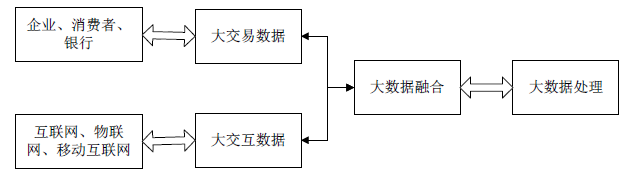
\includegraphics[width=0.8\textwidth]{Figures/data.png}
\end{generalfig}

引用该图片例如:\autoref{fig:data}。请注意generalfig第一个参数是标题,第二个参数是引用。

使用 minipage 排版并排插图。

\begin{figure}[htp!]
\begin{minipage}[h]{0.48\linewidth}
\centering
  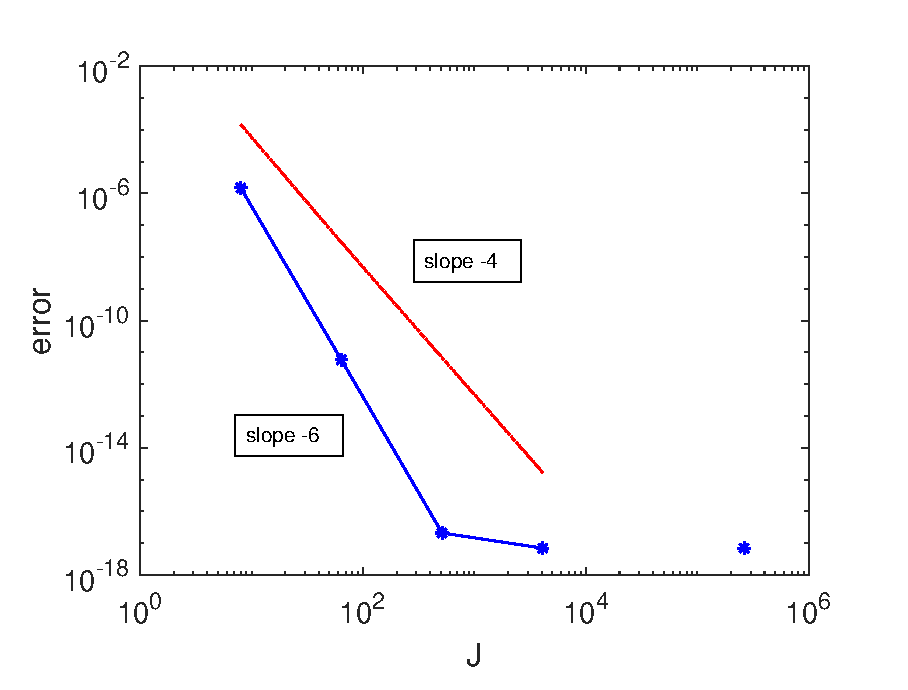
\includegraphics [height=2.5in]{Image1.eps}
    \caption{A方法的 $L^\infty$误差.}
    \label{fig:error1}
\end{minipage}
  \hfill\quad
\begin{minipage}[h]{0.48\linewidth}
\centering
   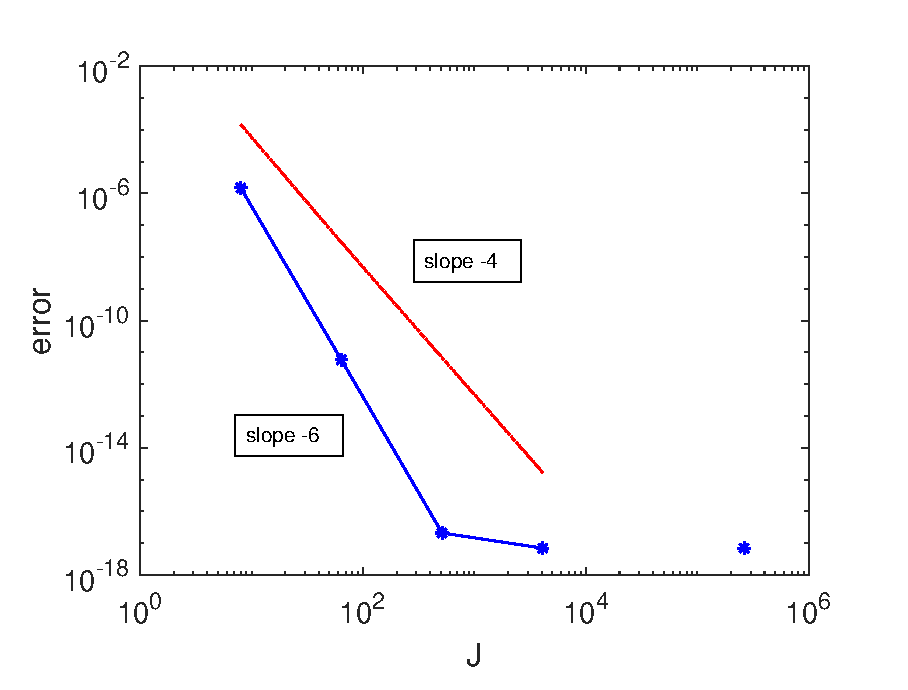
\includegraphics [height=2.5in]{Image1.eps}
   \caption{B方法的 $L^\infty$误差.}
   \label{fig:error2}
\end{minipage}
\end{figure}

引用图片:\autoref{fig:error1} 与 \autoref{fig:error2}

\chapter{列表的使用}

\section{计数列表}

这是一个计数的列表
\begin{enumerate}
	\item 第一项
		\begin{enumerate}
			\item 第一项中的第一项
			\item 第一项中的第二项
		\end{enumerate}
	\item 第二项
	\item 第三项
\end{enumerate}



\section{不计数列表}

这是一个不计数的列表
\begin{itemize}
	\item 第一项
	\begin{itemize}
		\item 第一项中的第一项
		\item 第一项中的第二项
	\end{itemize}
	\item 第二项
	\item 第三项
\end{itemize}


%%%%%%%%%%%%%%%%%%%%%%%% 生成参考文献  %%%%%%%%%%%%%%%%%%%%%%%%%%%%%%%%%%%%%%

%使用方法:\bibliography{参考文件1文件名, 参考文献2文件名, ...}
\nocite{*}  % 可以显示全部参考文献,包括未引用的
\bibliography{mybib}



%%%%%%%%%%%%%%%%%%%%%% 攻读硕士学位期间的研究成果  %%%%%%%%%%%%%%%%%%%%%%%%%%%
\begin{researchpage}
%\pagestyle{plain} \Appendix{


\noindent[1] {{\bf Author1} and Author2},  {\em The name of the published article 1}, {\bf Name of Journal}, 01 (2020), 1001-1008.


\noindent[2] {{\bf Author1},  Author2 and Author3},  {\em The name of the published article 2}, submitted to
Journal of XXX.


\end{researchpage}



%%%%%%%%%%%%%%%%%%%%%%%%%%% Thanks page %%%%%%%%%%%%%%%%%%%%%%%%%%%%%%%%%%%%

\begin{thankpage}
\setlength{\baselineskip}{24pt}

感谢老师感谢老师感谢老师感谢老师感谢老师感谢老师感谢老师感谢老师感谢老师感谢老师感谢老师感谢老师感谢老师感谢老师感谢老师感谢老师感谢老师感谢老师感谢老师感谢老师感谢老师感谢老师感谢老师感谢老师感谢老师感谢老师感谢老师感谢老师感谢老师感谢老师感谢老师感谢老师感谢老师感谢老师感谢老师感谢老师
		
感谢老师感谢老师感谢老师感谢老师感谢老师感谢老师感谢老师感谢老师感谢老师感谢老师感谢老师感谢老师感谢老师感谢老师感谢老师感谢老师感谢老师感谢老师感谢老师感谢老师感谢老师感谢老师感谢老师感谢老师感谢老师感谢老师

感谢老师感谢老师感谢老师感谢老师感谢老师感谢老师感谢老师感谢老师感谢老师感谢老师感谢老师感谢老师感谢老师感谢老师感谢老师感谢老师感谢老师感谢老师感谢老师感谢老师感谢老师感谢老师感谢老师感谢老师感谢老师感谢老师感谢老师感谢老师感谢老师感谢老师感谢老师感谢老师感谢老师感谢老师感谢老师感谢老师

\end{thankpage}


%\backmatter %结束章节自动编号
% 添加附录
%\appendix
%\chapter{附录 这是第一个附录}
%\section*{附录可以有小节}
%这里是附录环境,其中的section、subsection、subsubsection已经变为附录的样式,并且会以这种样式加入目录中
%
%\chapter{附录 B ~~ 这是第二个附录}

	
\end{document} 